\documentclass[tikz,border=8pt]{standalone}
\usepackage{amsmath,amssymb}
\usetikzlibrary{arrows.meta,calc,decorations.markings,decorations.pathmorphing,patterns,shapes.geometric,positioning}

\begin{document}
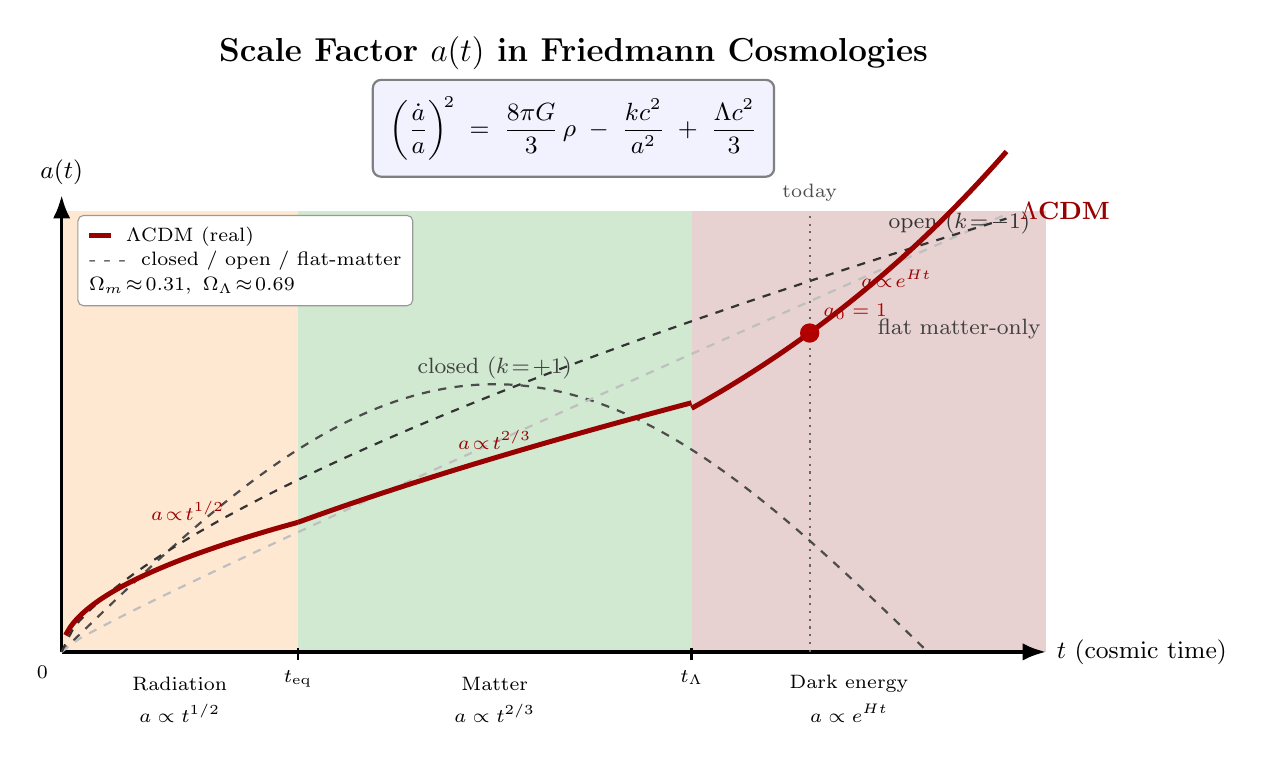
\begin{tikzpicture}[>=Latex, x=1cm, y=1cm,
  axis/.style={->, very thick, black},
  era/.style={opacity=0.18},
  curve/.style={very thick},
  ref/.style={thick, gray!70!black, dashed},
  lbl/.style={font=\footnotesize}]

  % --- Title at the top ----------------------------------------------------
  \node[font=\large\bfseries, align=center] at (6.5, 7.6) {%
    Scale Factor $a(t)$ in Friedmann Cosmologies};

  % --- Embedded equation banner --------------------------------------------
  \node[draw=black!50, thick, rounded corners=3pt, fill=blue!5,
        inner sep=6pt, align=center, font=\small] at (6.5, 6.65) {%
    $\displaystyle \left(\frac{\dot a}{a}\right)^{\!2}
       \;=\; \frac{8\pi G}{3}\,\rho \;-\; \frac{k c^{2}}{a^{2}}
       \;+\; \frac{\Lambda c^{2}}{3}$};

  % --- Era shading (background time-bands) ---------------------------------
  % radiation era
  \fill[orange, era] (0,0) rectangle (3.0, 5.6);
  % matter era
  \fill[green!50!black, era] (3.0,0) rectangle (8.0, 5.6);
  % Lambda era
  \fill[red!50!black, era] (8.0,0) rectangle (12.5, 5.6);

  % era labels at bottom
  \node[font=\scriptsize, align=center] at (1.5, -0.40) {Radiation};
  \node[font=\scriptsize, align=center] at (5.5, -0.40) {Matter};
  \node[font=\scriptsize, align=center] at (10.0, -0.40) {Dark energy};
  \node[font=\scriptsize, align=center] at (1.5, -0.78) {$a\propto t^{1/2}$};
  \node[font=\scriptsize, align=center] at (5.5, -0.78) {$a\propto t^{2/3}$};
  \node[font=\scriptsize, align=center] at (10.0, -0.78) {$a\propto e^{Ht}$};

  % --- Axes ---------------------------------------------------------------
  \draw[axis] (0,0) -- (12.5, 0) node[right, font=\small] {$t$ (cosmic time)};
  \draw[axis] (0,0) -- (0, 5.8) node[above, font=\small] {$a(t)$};
  \node[font=\scriptsize, anchor=north east] at (-0.05, -0.05) {$0$};

  % era boundary tick marks on x-axis
  \draw[thick] (3.0, 0.05) -- (3.0, -0.10) node[below, font=\scriptsize] {$t_{\rm eq}$};
  \draw[thick] (8.0, 0.05) -- (8.0, -0.10) node[below, font=\scriptsize] {$t_{\Lambda}$};

  % present-time marker
  \draw[thick, dotted, black!60] (9.5, 0) -- (9.5, 5.6);
  \node[font=\scriptsize, anchor=south, black!70] at (9.5, 5.6) {today};

  % --- Reference curve: closed (k=+1, recollapses) -----------------------
  % half-cycloid: rises then falls back to zero
  \draw[ref, gray!60!black] plot[domain=0:11, samples=80, smooth]
    ({\x}, {3.4*sin( deg(\x*0.2856) )});
  \node[lbl, gray!50!black] at (5.5, 3.6) {closed ($k\!=\!+1$)};

  % --- Reference curve: open (k=-1, ever-expanding decelerating) -------
  % a(t) ~ t  for k=-1  (linear late-time)  -- light gray
  \draw[ref, gray!50] plot[domain=0:12, samples=60, smooth]
    ({\x}, {0.42*\x + 0.15*sqrt(\x)});
  \node[lbl, gray!40!black] at (11.4, 5.45) {open ($k\!=\!-1$)};

  % --- Reference curve: flat matter-only (k=0, Lambda=0) ---------------
  % a(t) ~ t^{2/3}
  \draw[ref, gray!40!black] plot[domain=0:12, samples=80, smooth]
    ({\x}, {1.05*pow(\x, 0.6667)});
  \node[lbl, gray!50!black] at (11.4, 4.10) {flat matter-only};

  % --- MAIN curve: realistic LambdaCDM -----------------------------------
  % piecewise:
  %   t in [0,3]: radiation, a ~ t^{1/2}
  %   t in [3,8]: matter,    a ~ t^{2/3}, with continuity
  %   t in [8,12]: Lambda,   a ~ exp(H*t), with continuity
  \draw[curve, red!60!black, line width=1.8pt]
    plot[domain=0.05:3.0, samples=50, smooth]
      ({\x}, {0.95*sqrt(\x)});
  \draw[curve, red!60!black, line width=1.8pt]
    plot[domain=3.0:8.0, samples=70, smooth]
      ({\x}, {0.95*sqrt(3.0) * pow(\x/3.0, 0.6667)});
  % at t=8: a8 = 0.95*sqrt(3)*pow(8/3, 2/3) approx 0.95*1.732*1.881 approx 3.094
  \draw[curve, red!60!black, line width=1.8pt]
    plot[domain=8.0:12.0, samples=80, smooth]
      ({\x}, {3.094 * exp(0.18*(\x-8.0))});

  % main curve label
  \node[font=\small\bfseries, red!60!black, anchor=west] at (12.05, 5.6) {%
    $\Lambda$CDM};

  % main curve segment annotations
  \node[font=\scriptsize, red!60!black, anchor=south] at (1.6, 1.55) {%
    $a\!\propto\!t^{1/2}$};
  \node[font=\scriptsize, red!60!black, anchor=south] at (5.5, 2.45) {%
    $a\!\propto\!t^{2/3}$};
  \node[font=\scriptsize, red!60!black, anchor=south] at (10.6, 4.50) {%
    $a\!\propto\!e^{Ht}$};

  % marker dot for present time on main curve at t=9.5
  % a(9.5) = 3.094 * exp(0.18*1.5) = 3.094 * exp(0.27) approx 3.094*1.310 approx 4.05
  \fill[red!70!black] (9.5, 4.05) circle (3.5pt);
  \node[font=\scriptsize, red!70!black, anchor=south west] at (9.55, 4.10) {$a_0 = 1$};

  % --- Legend (top-left corner) -----------------------------------------
  \node[draw=black!40, rounded corners=2pt, fill=white,
        inner sep=4pt, align=left, font=\scriptsize, anchor=north west]
       at (0.20, 5.55) {%
    \textcolor{red!60!black}{\rule[0.4ex]{8pt}{1.8pt}}~ $\Lambda$CDM (real)\\[1pt]
    \textcolor{gray!60!black}{- - -}~ closed / open / flat-matter\\[1pt]
    \scriptsize $\Omega_m\!\approx\!0.31,\ \Omega_\Lambda\!\approx\!0.69$};

\end{tikzpicture}
\end{document}
